\section{Veruchsaufbau}
\label{sec:Veruchsaufbau}

\begin{figure}[htbp]
    \centering
    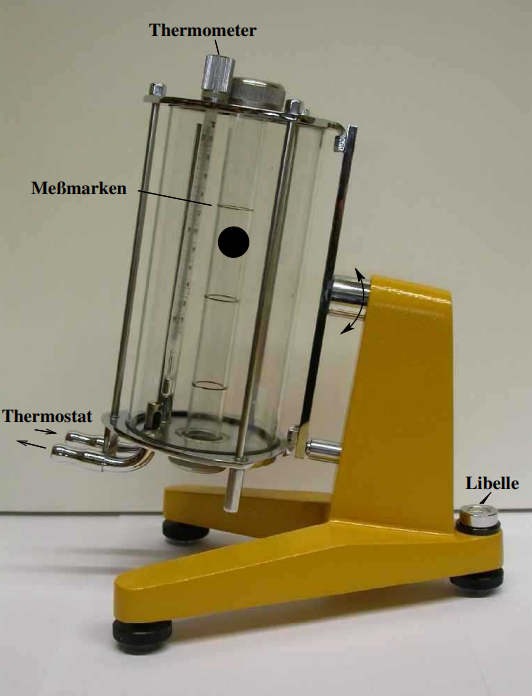
\includegraphics[width=0.7\textwidth]{bilder/hoeppler_viskosimeter.png}
    \caption{Höppler-Viskosimeter}
    \label{fig:hoeppler}
\end{figure}

Für die Versuchsdurchführung wird ein Kugelfall-Viskosimeter nach Höppler benötigt. Das Viskosimeter besteht aus einem Zylinder, in den Wasser eingefüllt ist. 
In diesen ist zentral eine Röhre mit drei Messmarkierungen im Abstand von $5\;\unit{cm}$ eingefasst. 